\section {Analysis}\label{sec:analysis}

Next, we conduct multiple case studies aimed at identifying common errors and exposing vulnerabilities in \judgemodels.
Specifically, we study the precision and recall of the \judgemodels (\cref{sec:analysis:subsec:precision_recall}), their ability to recall specific error types (\cref{sec:analysis:subsec:error_analysis}),  the suitability of using \judgemodels for instruction tuned models when compared with base models (\cref{sec:analysis:subsec:basevschat})
% \dieuwke{list what we investigate and provide section numbers}
, how responsive \judgemodels are to the length of prompts and the clarity of guidelines (\cref{sec:analysis:subsec:instructions}) and the leniency of \judgemodels in grading. (\cref{sec:analysis:quantifyingbias}).  
%\dieuwke{insert rest of the results}.

\subsection{Better aligned models have better recall, but not precision}
\label{sec:analysis:subsec:precision_recall}

First, we investigate the precision and recall of the \judgemodels, using the human judgement as gold standard.
We plot both -- maintaining the ordering of \cref{fig:llmalignment} -- in \cref{fig:precisionrecall}.
In the figure, we see that precision stays relatively constant; there is no clear relationship between alignment and how many false positives are predicted, which can be further observed in \cref{fig:confusionmatrix}.
The recall, on the other hand, shows a clear increasing trend: more aligned models have comparatively fewer false negatives.

\begin{figure}[h]
    \begin{subfigure}[b]{0.5\textwidth}
    \centering
        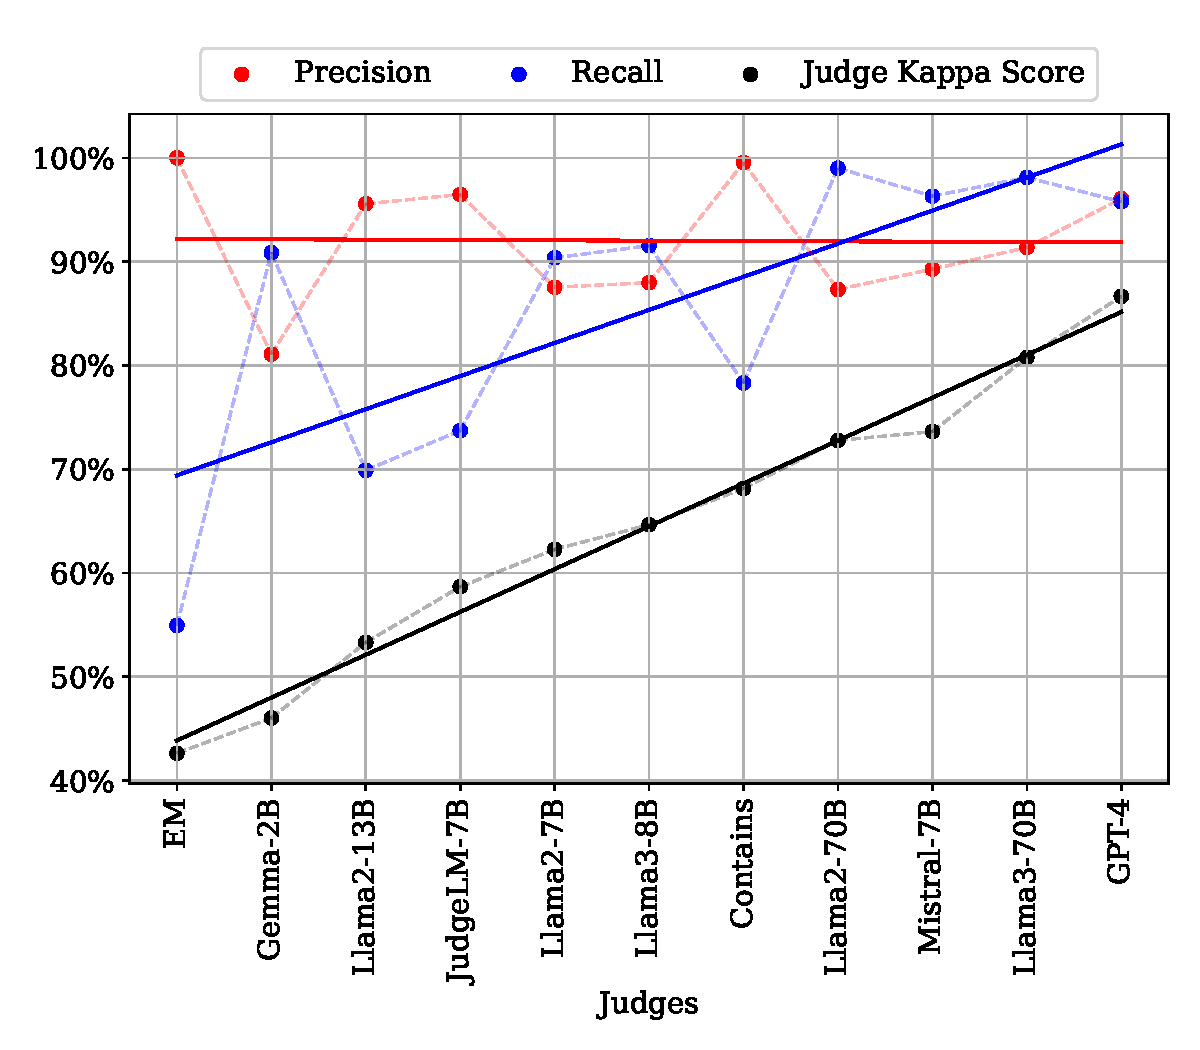
\includegraphics[width=\linewidth]{figures/PrecisionRecall_V5.pdf}
        \caption{}
        \label{fig:precisionrecall}
    \end{subfigure}
    \begin{subfigure}[b]{0.5\textwidth}
    \centering
        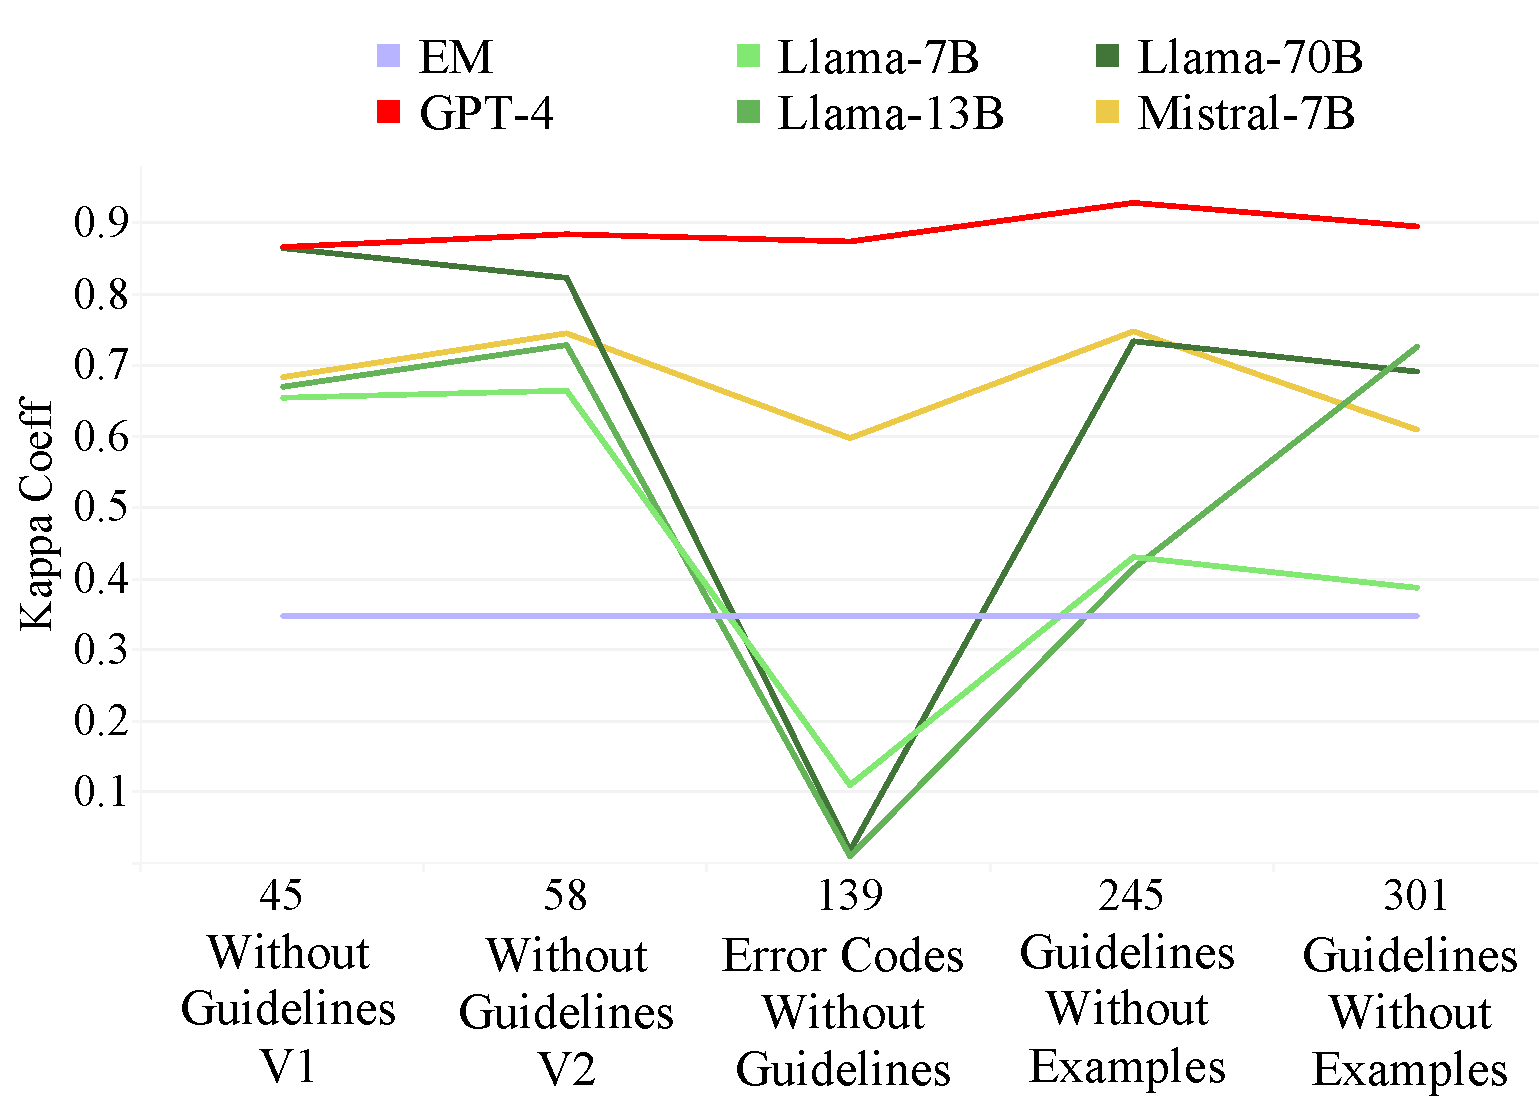
\includegraphics[width=\linewidth]{figures/TooMuchInfo.pdf}
        \caption{}
        \label{fig:TooMuchInfo}
    \end{subfigure}
    \caption{(a) Precision (\( R^2 \) = 0.0003) and recall (\( R^2 \) = 0.55) with increasing human alignment (\( R^2 \) = 0.98) (b) Cohen's Kappa coefficient (human alignment) vs Prompt token size for \JudgeModels
    \dieuwke{Should increase the font sizes on this one, put the legends on the top and afterwards align appropriately.}}
\end{figure}

% \begin{figure}[h]
%     \centering
%         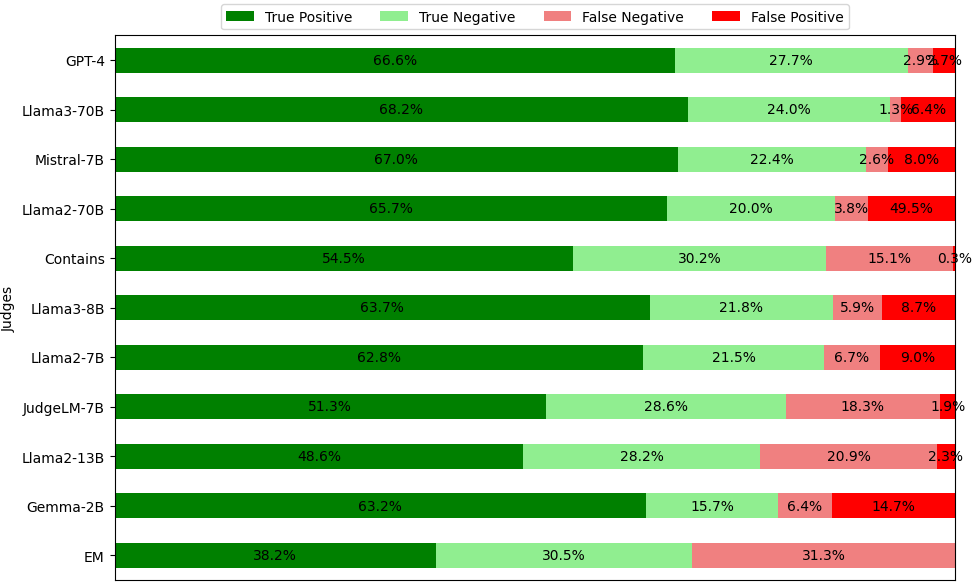
\includegraphics[width=\linewidth]{figures/ConfusionMatrixV2.png}
%         \caption{Judge performance \& error rate with increasing human alignment }
%         \label{fig:confusionmatrix}
% \end{figure}

\subsection{What types of errors do \judgemodels recall?}\label{sec:analysis:subsec:error_analysis}

\begin{table}[ht]
\resizebox{\textwidth}{!}{
    \begin{tabular}{lllll}
        Error code & Explanation & Example & Proportion & GPT-4 Recall\\ 
        \toprule\toprule
        \textbf{Incorrect entity} & \specialcell{Response refers to a wrong entity} & \specialcell{\texttt{Henry VII, Henry VIII, Edward VI,} \\ \texttt{Mary I and Elizabeth I}} & 86.9\% & 84.7\%\\
        \hline
        \textbf{Under-specified} & \specialcell{Response contains only part \\ of the answer} & \specialcell{\texttt{Henry VII, Henry VIII, Edward,} \\ \texttt{Mary, and Elizabeth}} & 10.6\% & 33.9\%\\
        \hline
        \textbf{Too few entities} & \specialcell{Response contains too few entities} & \specialcell{\texttt{Henry VII, Edward VI,} \\ \texttt{Mary I and James I}} & 2.47\% & 67.7\% \\
        \hline
        \textbf{Too many entities} & \specialcell{Response contains too many entities} & \specialcell{\texttt{Henry VII, Henry VIII, Edward VI,} \\ \texttt{Mary I, James I, and Elizabeth I}} & 2.7\% & 84.7\% \\
        \hline
        \textbf{Other} & \specialcell{Response is incorrect but cannot \\ be put into any of the above buckets} & \specialcell{\texttt{I'm sorry but I do not know the} \\ \texttt{answer to that question}} & 1.23\% & 16.9\% \\
        \bottomrule
    \end{tabular}
    }
    \caption{Error codes used to identify the types of errors made by \evaluatormodels when answering questions. The example question in this case is \texttt{``Excluding Lady Jane Grey, who were the five monarchs of the House of Tudor?''}, with the correct answer being \texttt{``Henry VII, Henry VIII, Edward VI, Mary I and Elizabeth I''}}\label{table:error_codes}
\end{table}

Next, we do an analysis of the types of errors that the \judgemodels are making, focusing on the best two \judgemodels: \judge{GPT-4} and \judge{Llama3-70B}.
To do so, we collect 900 outputs of \eval{Llama-7B} and annotate each question with an error code.
Then, we consider what percentage of those types of errors is correctly judged by the two judge models.
An overview of the error codes we considered can be found in \cref{table:error_codes}

In \cref{fig:precisionrecall}, we can see that \judge{GPT-4} has comparatively high recall when the answers refer to an incorrect entity, or too many entities are present.
It's recall for too few entities is also relatively high, while it drops substantially for under-specified answers and other error codes, suggesting that \judge{GPT-4} is more lenient with such mistakes.
\dieuwke{TODO: insert results for Llama3-70-B chat as well.}

% From this case study, we can see that 87\% of incorrect responses were because of knowledge gap of evaluation model. 
% Using GPT-4 Judge LLM, we evaluate each of the responses and then calculate the recall of each error code. From \cref{fig:recallfpr}, we observe that GPT-4 accurately recalls incorrect entities, too many entities, and too few entities. 
% However, GPT-4's recall drops to 20\% - 20\% for underspecified and other error codes indicating that it may be lenient with such error codes.
% 
% \begin{figure}[h]
%     \begin{subfigure}[b]{0.49\linewidth}
%         \centering
%         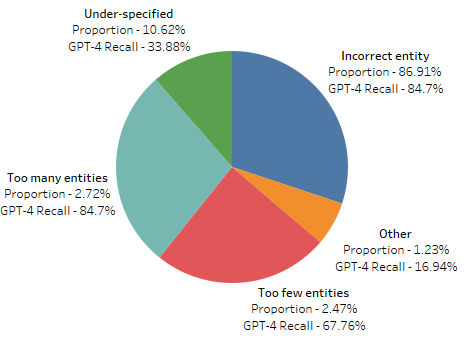
\includegraphics[width=\linewidth]{figures/ErrorCodeAnalysisV2.png}
%         \caption{\judge{GPT-4}}
%         \label{fig:recallfpr}
%     \end{subfigure}
%     \begin{subfigure}[b]{0.49\linewidth}
%         \centering
%         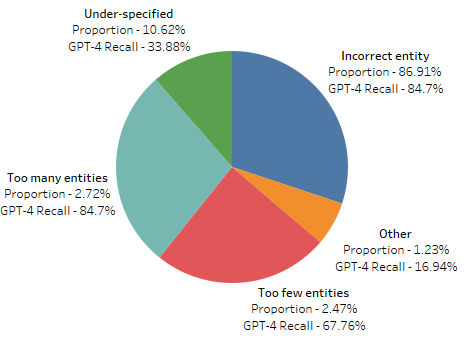
\includegraphics[width=\linewidth]{figures/ErrorCodeAnalysisV2.png}
%         \caption{\judge{Llama3-70B-Chat}}
%         \label{fig:recallfpr}
%     \end{subfigure}
%     \caption{Recall of specific errors by \judge{GPT-4} and \judge{Llama3-70B-chat}. 
%     `Proportion' indicates how many of the observed errors were of that specific type.
%     \dieuwke{Create Llama 3 plot on the right.}}
% \end{figure}

% \begin{figure}
%     \centering
%     \begin{subfigure}[b]{0.42\textwidth}
%         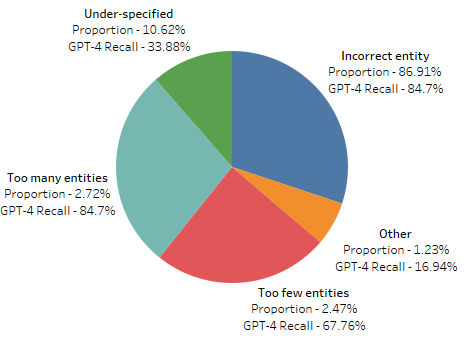
\includegraphics[width=\textwidth]{figures/ErrorCodeAnalysisV2}
%         \caption{}\label{fig:generalisation_over_time_c}
%     \end{subfigure}
%     \caption{}\label{fig:generalisation_over_time}
% \end{figure}

% To understand the pattern in judge LLM incorrect annotations, we run evaluation model Llama-7B on 900 samples and annotate each question with an error code.
% Based on our human annotation guidelines in \cref{sec:experiments:baselineandhumanannotation}, the different error codes are as defined below. 
% We provide examples in \cref{appendix:erroranalysis}. 
% \begin{itemize}
%     \item \textbf{Incorrect entity}: When response is incorrect based on knowledge reasoning.
%     \item \textbf{Under-specified}: When response is incorrect because it has partial information.
%     \item \textbf{Too few entities}: When the response was expected to have multiple entities but LLM responded with only a subset of references.
%     \item \textbf{Too many entities}: When the response was expected to have multiple entities but LLM responded with entities that are not part of the references.
%     \item \textbf{Other}: When response is incorrect but cannot be put into any of the above buckets.
% \end{itemize}

% \begin{figure}[H]
%     \centering
%     \begin{minipage}[t]{\textwidth}
%         \centering
%         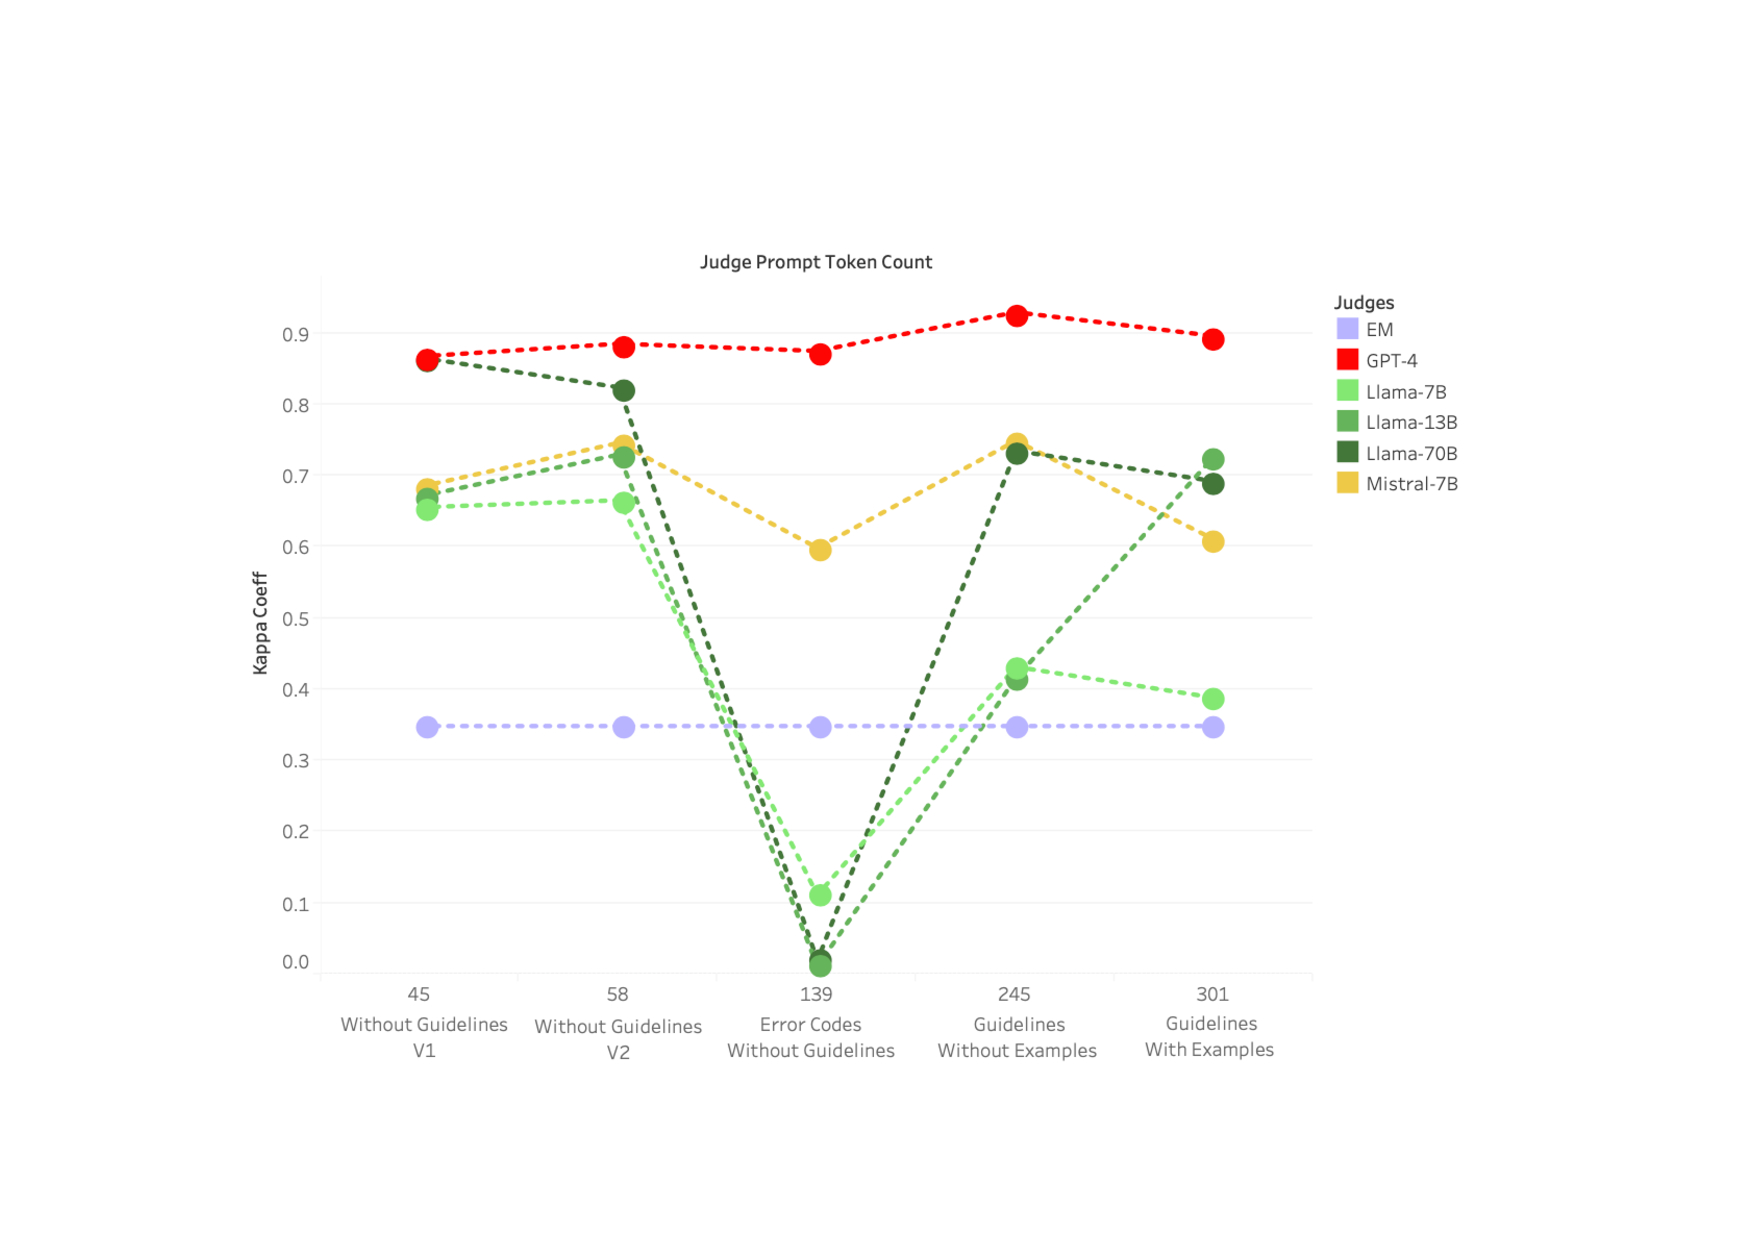
\includegraphics[width=1\textwidth, height=\textheight, keepaspectratio]{figures/TooMuchInfo_Scaled.pdf}
%         \caption{Cohen's Kappa score (human alignment) vs prompt token size for judge LLMs}
%         \label{fig:TooMuchInfo}
%     \end{minipage}
% \end{figure}
\subsection{Base vs Chat analysis} \label{sec:analysis:subsec:basevschat}

% \begin{table}[ht]
% \centering
% \vspace{0.5em} % Adjust the spacing here
% \begin{tabular}{ccccc}
% \multicolumn{1}{c}{\rule{0pt}{1em}} & \multicolumn{1}{c}{\rule{0pt}{1em}\judge{Human}} & \multicolumn{1}{c}{\rule{0pt}{1em}\judge{GPT}} & \multicolumn{1}{c}{\rule{0pt}{1em}\judge{Llama2-70B}} & \multicolumn{1}{c}{\rule{0pt}{1em}\judge{Llama2-7B}}\\ \hline
% \toprule\toprule
% Llama 7B & \rule{0pt}{1em}6.75 & \rule{0pt}{1em}9.5 & \rule{0pt}{1em}4.75 & \rule{0pt}{1em}1.75\\ 
% \midrule
% Mistral 7B & \rule{0pt}{1em}10.75 & \rule{0pt}{1em}11.5 & \rule{0pt}{1em}7.5  & \rule{0pt}{1em}6.25\\
% \midrule
% Llama 13B & \rule{0pt}{1em}16.5 & \rule{0pt}{1em}9 & \rule{0pt}{1em}3.75 & \rule{0pt}{1em}3.75\\
% \midrule
% Llama 70B & \rule{0pt}{1em}10 & \rule{0pt}{1em}10.25 & \rule{0pt}{1em}10  & \rule{0pt}{1em}7 \\
% \bottomrule
% \end{tabular}
% \vspace{1em} % Adjust the spacing between caption and table
% \caption{Difference in Evaluation Scores between different Base - Chat \evaluatormodel pairs for different \judgemodels}
% \label{tab:BasevsChat}
% \end{table}

Here, we examine the differences in evaluation scores between Base and Chat model pairs and how these scores are assessed by different \judgemodels. The results in \cref{tab:BasevsChat} demonstrate that across all \judgemodels, the base models consistently outperform their respective chat \evaluatormodels
 
\begin{table}[ht]
\begin{minipage}[b]{0.49\linewidth}
    \centering
    \renewcommand{\arraystretch}{2.5}
    \resizebox{\textwidth}{!}{ % Adjusts the table to fit the text width
    \begin{tabular}{ | p{2cm} | p{1cm} | p{1cm} | p{1cm} | p{1cm} |}
        \hline
        Judge LLM & Human & GPT-4 & Llama2 & Llama2\\ 
        & & & 70B & 7B\\ \hline
        Llama2-7B & 6.75 & 9.5 & 4.75 & 1.75 \\ \hline
        Mistral-7B & 10.75 & 11.5 & 7.5 & 6.25 \\ \hline
        Llama-13B & 16.5 & 9 & 3.75 & 3.75 \\ \hline
        Llama-70B & 10 & 10.25 & 10 & 7 \\ \hline
    \end{tabular}}
    \caption{Difference in Evaluation Scores between different Base - Chat evaluatormodel pairs for different judgemodels}
    \label{tab:BasevsChat}
\end{minipage}
\begin{minipage}[b]{0.49\linewidth}
\centering
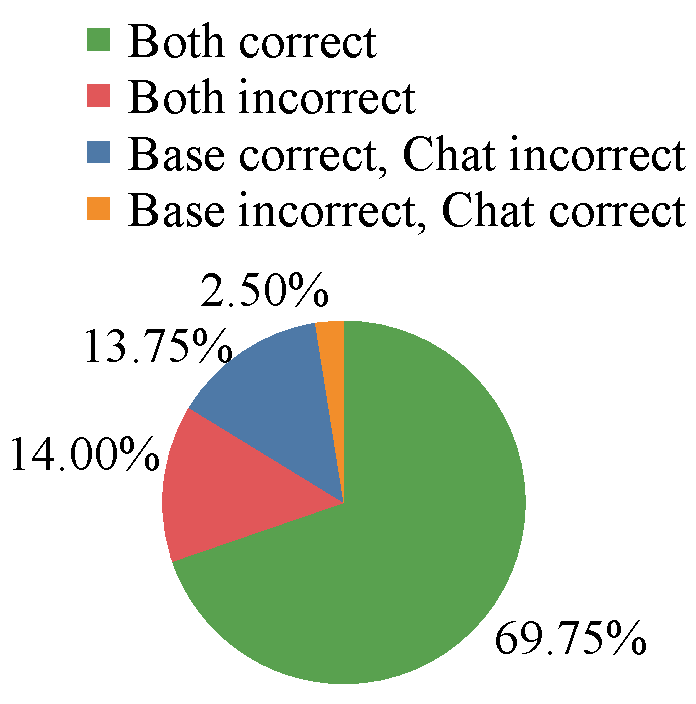
\includegraphics[width=\linewidth]{figures/PieChart.pdf}
\captionof{figure}{Pie chart showing the percentage of questions categorized by the judgement from Base and Chat models.}
\label{fig:comparisonPieChart}
\end{minipage}
\end{table}

% \begin{figure}[H]
%     \begin{subfigure}[t]{0.49\textwidth}
%         % Table LaTeX code
%         \centering
%         \begin{tabular}{ccccc}
%             \multicolumn{1}{c}{\rule{0pt}{1em}} & \multicolumn{1}{c}{\rule{0pt}{1em}\judge{Human}} & \multicolumn{1}{c}{\rule{0pt}{1em}\judge{GPT}} & \multicolumn{1}{c}{\rule{0pt}{1em}\judge{Llama2-70B}} & \multicolumn{1}{c}{\rule{0pt}{1em}\judge{Llama2-7B}}\\ \hline
%             \toprule\toprule
%             Llama 7B & \rule{0pt}{1em}6.75 & \rule{0pt}{1em}9.5 & \rule{0pt}{1em}4.75 & \rule{0pt}{1em}1.75\\ 
%             \midrule
%             Mistral 7B & \rule{0pt}{1em}10.75 & \rule{0pt}{1em}11.5 & \rule{0pt}{1em}7.5  & \rule{0pt}{1em}6.25\\
%             \midrule
%             Llama 13B & \rule{0pt}{1em}16.5 & \rule{0pt}{1em}9 & \rule{0pt}{1em}3.75 & \rule{0pt}{1em}3.75\\
%             \midrule
%             Llama 70B & \rule{0pt}{1em}10 & \rule{0pt}{1em}10.25 & \rule{0pt}{1em}10  & \rule{0pt}{1em}7 \\
%             \bottomrule
%         \end{tabular}
%         \caption{}
%         \label{fig:comparisonTable}
%     \end{subfigure}
%     \begin{subfigure}[t]{0.49\textwidth} % Adjusted width
%         \centering
%         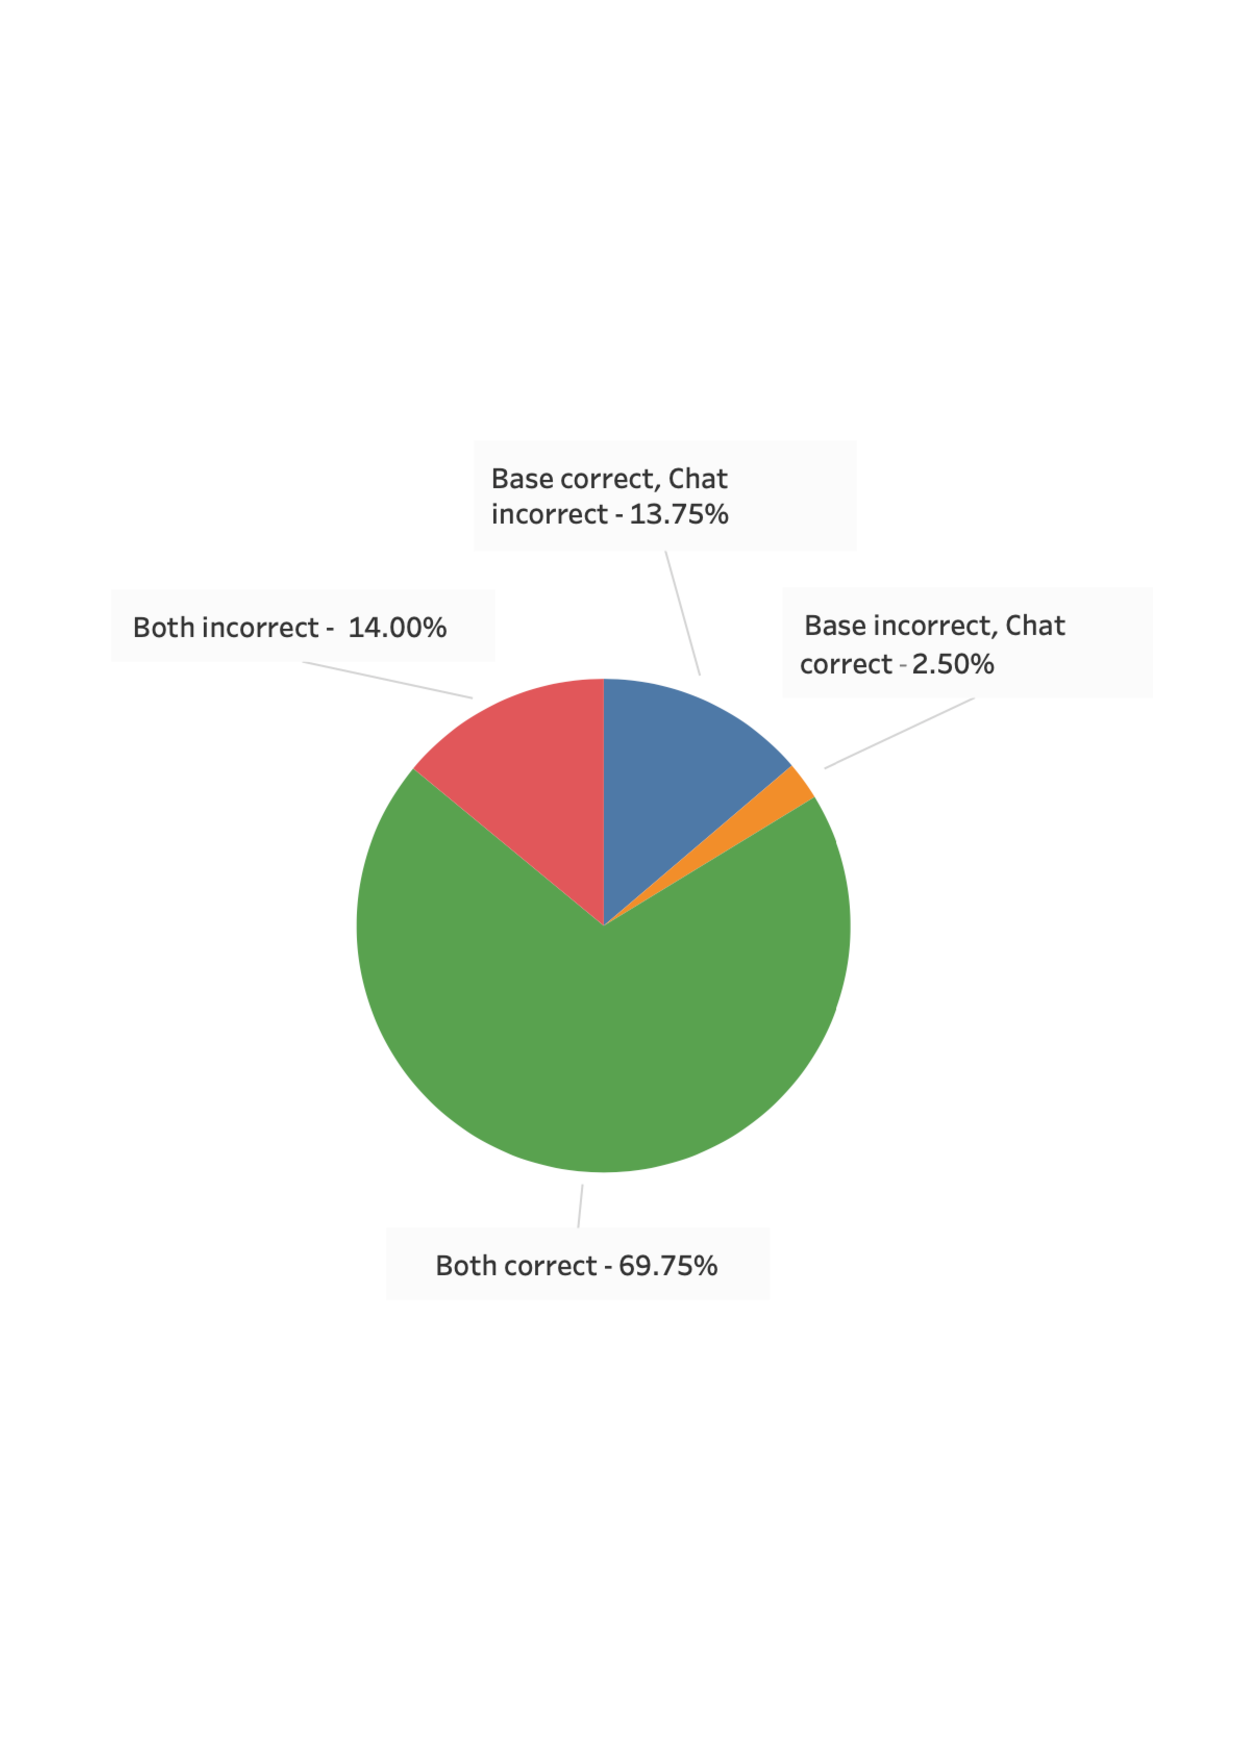
\includegraphics[width=\linewidth]{figures/Error_codes_piechart.pdf}
%         \caption{}
%         \label{fig:comparisonPieChart}
%     \end{subfigure}
%     \caption{(a) Evaluation scores comparison in tabular format for different Base-Chat \evaluatormodel pairs for different \judgemodels. (b) Pie chart showing the percentage of questions categorized by the judgement from Base and Chat models.}
%     \label{fig:BasevsChatErrorPlots}
% \end{figure}
 
% \begin{figure}[H]
%     \begin{subfigure}[t]{0.57\textwidth}
%         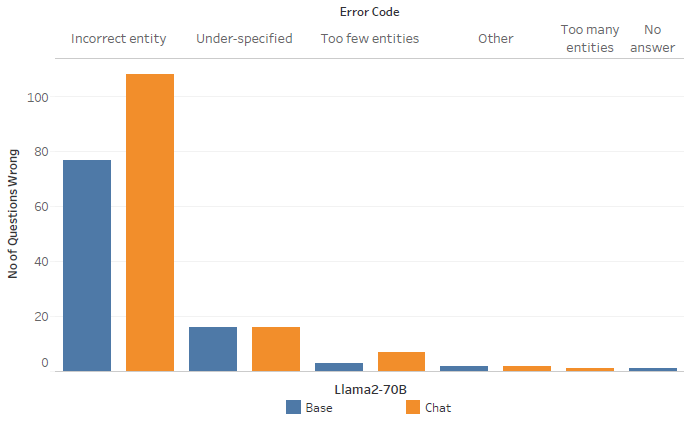
\includegraphics[width=\linewidth]{figures/Error_Codes_BarPlot.png}
%         \caption{}
%         \label{fig:comparisonBarplot}
%     \end{subfigure}
%     \hspace{0.03\textwidth}
%     \begin{subfigure}[t]{0.42\textwidth}
%         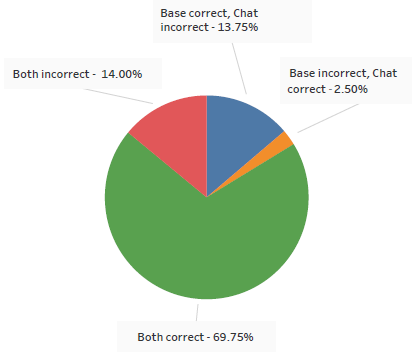
\includegraphics[width=\linewidth]{figures/Error_codes_piechart.png}
%         \caption{}
%         \label{fig:comparisonPieChart}
%     \end{subfigure}
%     \caption{(a)Incorrect questions count by error codes for \eval{Llama2 70B} Base vs Chat models
%     (b) Pie chart showing the percentage of questions categorized by the judgement from Base and Chat models.}
%     \label{fig:BasevsChatErrorPlots}
% \end{figure}

Let us assume the difference in the score of Base and Chat models is because of the following factors:

\begin{itemize}[noitemsep]
\item Knowledge unlearning by the chat models or Loss in knowledge (Correct Answer by Base model and Wrong Answer by Chat model) - $\mathcal{L}_{knowledge}$
\item Error in judgement by \judgemodels (Right answer by Chat model but wrong judgement or Wrong answer by Base model but judged as right) - $\epsilon$
\item Misc (Chat model fails to understand the prompt or answer Cut off) - $\mu$
\end{itemize}

\[
\begin{array}{cc}
\Delta_{\text{Human}} = \mathcal{L}_{knowledge} + \mu & \hspace{2cm} \Delta_{\text{LLM}} = \mathcal{L}_{knowledge} + \mu \pm \epsilon
\end{array}
\]

%%%%%%%%%%%%%%%%%%%%%%%%%
% Storyline
% 1) First we show the difference in scores and show not many 'Answer cut off' or other errors for chat models and hence its mostly Knowledge unlearning that contributes to delta in scores between Base and Chat models
% 2) Then we have to explain why is the delta varying across all judge models since Knowledge unlearning is same no matter what judge model we use. So here we say that its upto the judge model. Bigger judge = lineant scoring, smaller judge = harsher. Hence decrease in delta. Additionally, Knowledge unlearning is greater in bigger Base-Chat pairs
%%%%%%%%%%%%%%%%%%%%%%%%%%

Assuming there is zero error in human judgement, $\epsilon$ in $\Delta_{\text{Human}}$ = 0. 

The plots in \cref{fig:comparisonPieChart} and \cref{fig:comparisonBarplot} suggest that there is some knowledge unlearning, as the Chat model provides more incorrect answers than the Base model, with the majority of these errors being classified as 'incorrect entities' or 'under specification'. Examples can be found in \cref{app:BaseVsChatSupp}

Furthermore, \cref{fig:BasevsChat} shows with an increase in model size, \judge{GPT} has a similar Kappa and alignment score with humans only for the Chat models. This implies that while bigger \judgemodels effectively parse and evaluate the verbose responses from the chat models, the main problem lies in the accuracy of their answers, which leads to a lower judge score and further suggesting knowledge unlearning.

% and the knowledge gap between the base and chat models is increasing with increase in \evaluatormodel size
% The absolute $\Delta_{\text{LLM}}$ and $\Delta_{\text{Human}}$ values increase as the \evaluatormodels size increases. However the knowledge gap between the Base-Chat pairs of larger models is greater than for smaller models.
Interestingly, across all \judgemodels, as the size of the \evaluatormodel increases, $\Delta$ also increases, suggesting that $\mathcal{L}_{knowledge}$ between the Base and Chat models widens as the model size grows.
% This discrepancy underscores the inadequacy of smaller \judgemodels as evaluators

Additionally, as the \judgemodel size gets smaller, the $\Delta_{\text{LLM}}$ values decreases, well beyond the observed $\Delta_{\text{Human}}$. Given that $\mathcal{L}_{knowledge}$ and $\mu$ remain constant across all the \judgemodels, the only variable changing here is $\pm \epsilon$. \cref{tab:eval-scores} reveals that both base and chat models are evaluated too strictly by the smaller \judgemodels, resulting in $\Delta_{\text{LLM}}$s that are smaller but absolute scores that deviate significantly from the true scores. 


\begin{figure}[h]
    \centering
    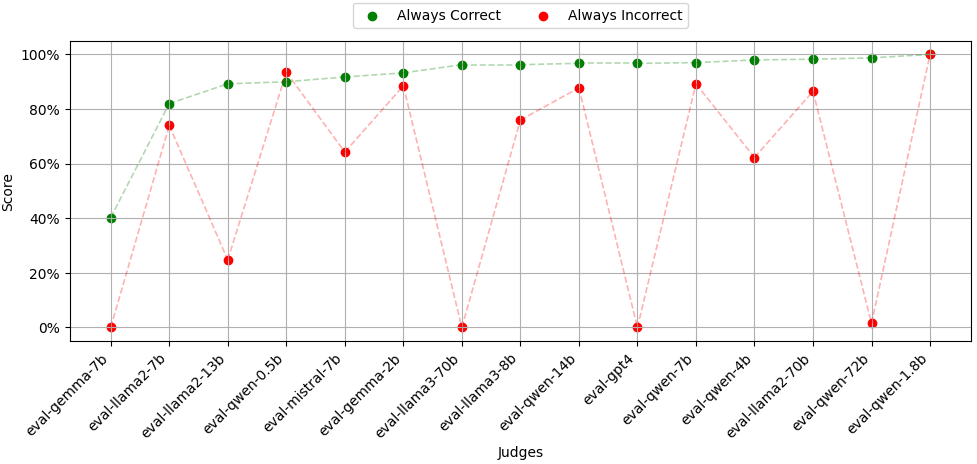
\includegraphics[width=\textwidth]{figures/Judgeguidelines.png}
    \caption{Performance of \judgemodels with constant response outputs \kc{Fig to be updated}}
    \label{fig:judge_dummy}
\end{figure}

% \begin{figure}[H]
%     \begin{minipage}[b]{0.49\textwidth}
%         \centering
%         \includegraphics[width=\textwidth]{figures/BasevsChat7b.png}
%         % \caption{Comparison Scores for Llama 7B Base and Llama 7B Chat}
%     \end{minipage}
%     \hfill
%     \begin{minipage}[b]{0.49\textwidth}
%         \centering
%         \includegraphics[width=\textwidth]{figures/BasevsChat70b.png}
%         % \caption{Comparison Scores for Llama 70B Base and Llama 70B Chat}
%     \end{minipage}
%     \caption{Comparison of Llama 7B and Llama 70B Models}
%     \label{fig:comparison}
% \end{figure}



% From these observations, we can draw the conclusions that

% 1) There is a knowledge gap between base and chat models which gets more prominent in bigger models. \\
% 2) The ideal LLM evaluator is more lenient than the smaller models and more stricter than GPT \\
% 3) Base models are subject to more relaxed judgement as compared to Chat models.

\subsection{\JudgeModel sensitivity to prompt length and quality}\label{sec:analysis:subsec:instructions}

% \textcolor{red}{Update with latest experiment V3-V4-Default-V2-V 1 trends. Bake everything into 1 plot.}
% \dieuwke{I am a bit confused about this subsection, to be discussed!}

Next, we study the impact of the prompt to the \judgemodels' ability to do accurate assessment.
Specifically, we investigate to what extent the precise instructions provided to the \judgemodel impact how it judges \evaluatormodels' answers.

We use five different prompt versions varying in length and specificity, with token counts excluding those from the question and references, focusing only on the instructions given to the \judgemodel during evaluation (see \cref{app:TMI} for prompt templates). Each prompt instructs the \judgemodels on evaluating responses, with complexity and detail increasing with token count. Error codes are introduced in the third smallest prompt (139 tokens, see \cref{app:error_codes_without_guidelines}) and elaborated with examples in the longer prompts.
% 
% \dieuwke{We need a bit more explanation of where these prompts come from and how they differ, plus a link to the full prompts in the appendix.}
% The aim was to observe how these variations affected the stringency of evaluation and to evaluate the sensitivity of the Judge LLM's performance to the prompt. 
% \textcolor{red}{Let's remove Llama 13B now as it's making the graph confusing}\\
% \textcolor{red}{Key Takeaway - Adding more instructions for Judges makes them more lineant}
% With an increase in the number of tokens in the prompt, resulting in higher complexity and detailed instructions for the judge to follow, the agreement between the judge LLM and human evaluation tends to decrease, as measured by the Cohen's Kappa score. 
% However, this trend does not apply to GPT-4, which maintains a high level of agreement with human evaluation even as the prompt complexity increases, and in fact gets a higher alignment with better instructions.

% For Human Guidelines V3, there is a decline in alignment as the prompt introduced the different types of errors that the judge could encounter,but without proper explanation that confused all the judge LLMs. However, in the subsequent bigger prompts, each error type was elaborated with examples to clear any ambiguity for the judge LLMs, which lead to a better performance.

From \cref{fig:TooMuchInfo}, it is evident that both \judge{Mistral-7B} and \judge{GPT-4} exhibit little variance in their Kappa agreement with humans based on the level of detail in the evaluation guidelines provided in the prompt. However, all the \judge{Llama-2} models perform worse as the prompt length and guideline complexity increase.

The \judgemodels are sensitive to the prompt. Prompt engineering to improve the evaluation performance of the \judgemodels has virtue but it has to be done carefully with experimentation and it highly depends on how the model reacts to it. Providing them with detailed instructions most often results in a worse performance as shown in \cref{fig:TooMuchInfo}. 

Interestingly, all the models except \judge{GPT-4} perform better with good kappa coefficient agreement with humans when using the simple prompt templates with no guidelines (\cref{app:default_v2(44)}) compared to using the prompts with the guidelines that the humans used while judging.(\cref{app:human_guidelines_v2(245)})

\textbf{\judge{GPT-4} has potential to achieve near \judge{human} performance by providing it with detailed guidelines and prompt refinement}. It reaches its best performance with a kappa coefficient of around 0.93 when detailed guidelines in the prompt, compared to 0.96 achieved between humans \cref{sec:experiments:baselineandhumanannotation} following the same guidelines. \textbf{Providing the other \judgemodels with detailed guidelines might confuse them}, but they have a strong base definition on how to evaluate the responses even without any extra information about the evaluation process.

% \subsection{Judge LLM's ability to follow grading instructions}\label{sec:analysis:subsec:judge-ability}

To test the ability of the \judgemodels in identifying responses, we run the benchmarks on five dummy models: the first three always respond with a constant output -- \texttt{``I don't know''}, \texttt{``Yes''}, and \texttt{``Sure''}, the fourth simply repeats the question back as its response, and the fifth always returns the correct response by returning one of the references as its answer. 
%
\cref{fig:judge_dummy} shows that while some \judgemodels are able to identify and correctly mark the incorrect dummy answers as incorrect (or correct in case of the fifth dummy model), some models, notably \judge{Llama-2 70B} that shows high alignment with human evaluations, incorrectly evaluates most of the questions.
%
We hypothesize that, given the references, while all but the smallest \judgemodels are able to correctly identify a plausible but incorrect response as being incorrect, \textbf{the \judgemodels can be confused if the response to a question to be evaluated is something completely unrelated to the questions}, in which case the \judgemodels might not be able to figure out which part of the prompt contains the response they are supposed to evaluate.

% \textcolor{red}{Definitely show adversarial}


\subsection{Leniency Bias}\label{sec:analysis:quantifyingbias}

% \textcolor{red}{Table and the Plot can be made side-by-side}

\begin{figure}[!htbp]
\begin{minipage}{0.45\textwidth}
   \begin{table}[H]
    \centering
    \label{tab:p-vals}
    \begin{tabular}{lrrr}
      \toprule
      Evaluator & $\kappa$ & $P_e$ & $P_+$ \\
      \midrule
      eval-qwen-1.8b & 0.19 & 0.18 & 1.00 \\
      eval-qwen-0.5b & 0.19 & 0.19 & 0.87 \\
      eval-gemma-7b & 0.40 & 0.32 & 0.07 \\
      eval-gemma-2b & 0.50 & 0.62 & 0.80 \\
      eval-qwen-4b & 0.69 & 0.67 & 0.89 \\
      eval-llama2-7b & 0.66 & 0.68 & 0.36 \\
      eval-mistral-7b & 0.72 & 0.75 & 0.75 \\
      eval-llama2-13b & 0.68 & 0.76 & 0.45 \\
      eval-llama2-70b & 0.80 & 0.79 & 0.94 \\
      eval-qwen-7b & 0.80 & 0.79 & 0.77 \\
      eval-llama3-8b & 0.81 & 0.80 & 0.84 \\
      eval-qwen-72b & 0.82 & 0.80 & 0.93 \\
      eval-qwen-14b & 0.83 & 0.82 & 0.83 \\
      eval-llama3-70b & 0.84 & 0.84 & 0.79 \\
      eval-gpt4 & 0.85 & 0.85 & 0.66 \\
      \bottomrule
    \end{tabular}
    \caption{Estimated values of $P_e$ and $P_+$ for different \judgemodels}
    \label{tab:pvals}
    \end{table}
    
  
\end{minipage}%
\hspace{1cm}
\begin{minipage}{0.45\textwidth}
  \centering
  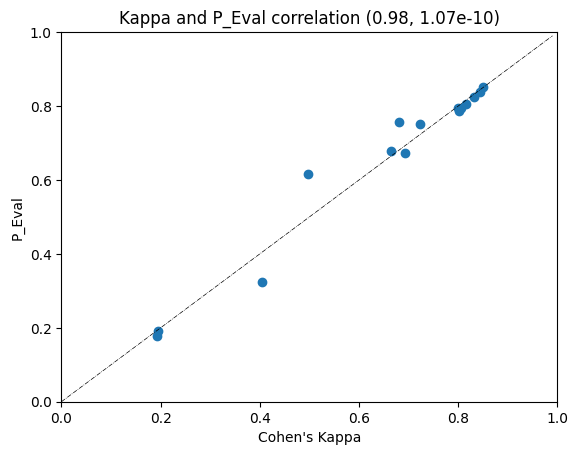
\includegraphics[width=\linewidth]{figures/eval-quality-kappa-correlation.png}
  \caption{Pearson's correlation coefficient between $\kappa$ and $P_e$ for \judgemodels.}
  \label{fig:k-p-corr}
\end{minipage}
\end{figure}


 

To estimate the inherent biases that might be present in the judge models, we present a simple hypothesis: For a given judge model and a given benchmark, the judge model correctly understands the task given to it and thus returns the correct evaluation with probability $P_e$. In the cases where the judge is not able to correctly understand the task, it randomly gives an evaluation of \texttt{true} with probability $P_+$, and an evaluation of \texttt{false} with the remaining probability of $1-P_+$.

The estimated probabilities using this method, with human evaluation as the reference, are shown in \cref{tab:pvals}. See Appendix XYZ for more details. We observe that the estimated evaluation probability $P_e$ is highly correlated to the Cohen's Kappa score of the judges, with a Person correlation coefficient of $0.98$, as shown in Fig. \cref{fig:k-p-corr}.

We observe that $P_+$ for most models is significantly higher than $0.5$, indicating a tendency of the judge models to evaluate a response as correct when they are not able to completely understand the prompt. 
% These biases are also observed in Section \cref{subsec:judge-ability}.

 
